\documentclass[twocolumn]{jsarticle}
\usepackage[dvipdfmx]{graphicx}
\usepackage{bm}
\usepackage{amsmath}
\usepackage{amssymb}
\usepackage{amsfonts}
\usepackage{comment}
\usepackage{listings}
\usepackage{cases}
\usepackage{siunitx}
\usepackage[hyphens]{url}
\lstset{
    basicstyle={\ttfamily},
    identifierstyle={\small},
    commentstyle={\smallitshape},
    keywordstyle={\small\bfseries},
    ndkeywordstyle={\small},
    stringstyle={\small\ttfamily},
    frame={tb},
    breaklines=true,
    columns=[l]{fullflexible},
    numbers=left,
    xrightmargin=0zw,
    xleftmargin=3zw,
    numberstyle={\scriptsize},
    stepnumber=1,
    numbersep=1zw,
    lineskip=-0.5ex,
    keepspaces=true,
    language=c
}
\renewcommand{\lstlistingname}{リスト}
\makeatletter
\newcommand{\figcaption}[1]{\def\@captype{figure}\caption{#1}}
\newcommand{\tblcaption}[1]{\def\@captype{table}\caption{#1}}
\makeatother

\title{6-3 IC温度センサー}
\author{Ec5 24番 平田 蓮}
\date{}

\begin{document}
\maketitle
\section{IC温度センサーとは?}
    IC(集積回路)温度センサーは温度に比例した出力電圧$\cdot$電圧を生成する。
    一般的な対応温度範囲は$-55〜150 \si{\degreeCelsius}$である。

    温度を検出する機能を持つセンサーにはサーミスタ、
    熱電対などがあるが、IC温度センサーは文字通りICで構成されている。

    IC温度センサーの中には、アナログ電圧または電流を出力するもの、
    デジタル信号を出力するものがある。
    デジタル出力の中には実際の温度を出力するものと、
    ある設定温度に対して温度がそれより高いか低いかの2値出力をする
    温度スイッチの役割を果たすものがある。

\section{構造・原理}
    \subsection{半導体の温度特性}
        予備知識として、ダイオードなどの半導体の温度特性に触れる。
        PN接合における順方向電圧は、温度に比例する特性がある。
        具体的には、一定の順電流のもとで、
        温度を上げるほど順方向電圧が低下する。

    \subsection{基本構造$\cdot$原理}
        IC温度センサーの基本構造を図\ref{fig:analog}に示す。

        \begin{figure}[h]
            \centering
            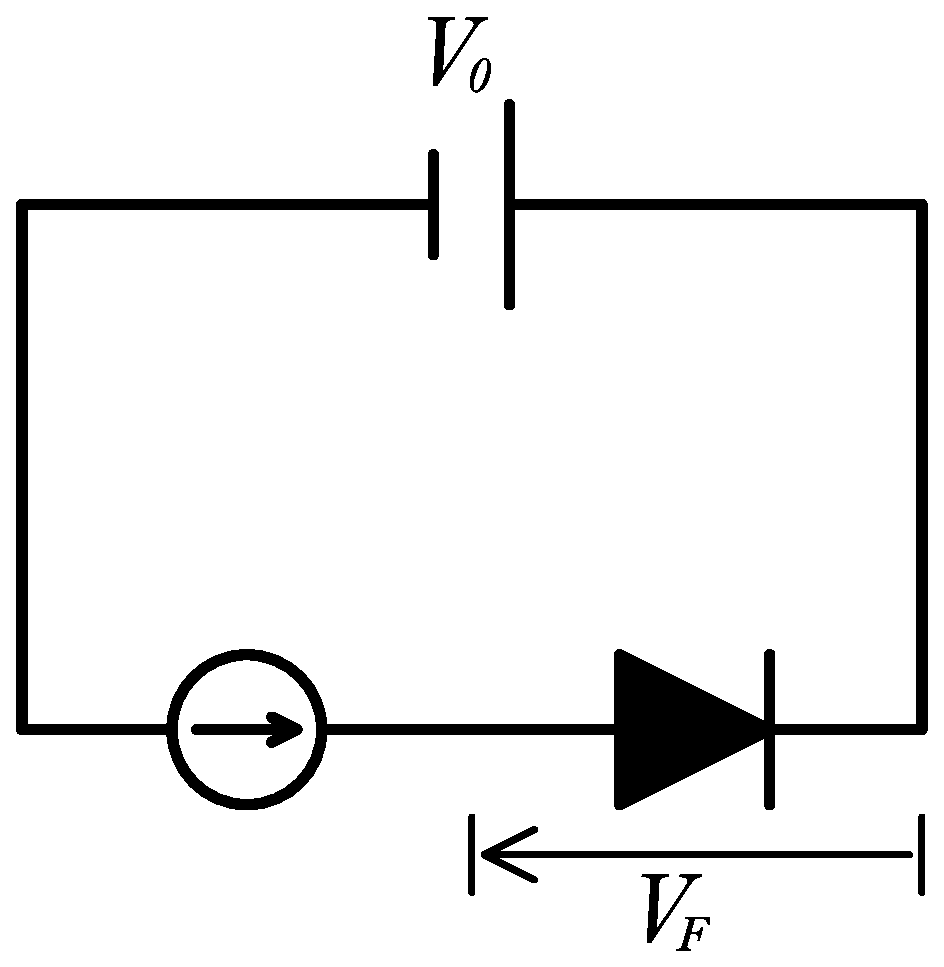
\includegraphics[width=0.6\hsize]{img/analog.eps}
            \caption{IC温度センサーの基本構造}
            \label{fig:analog}
        \end{figure}

        ダイオードの順方向電圧$V_F$を
        基準電圧である$V_0$と比較し、温度変化による電圧の変化を測定できる。
        
        アナログ出力を温度センサーは$V_F$をオペアンプに入力し、
        増幅した電圧や電流を出力する。
        デジタル信号を出力するタイプは、$V_F$をA/D変換し出力する。


        内部のダイオードには、主にシリコンダイオードが使用される。
        PNPトランジスタで代用も可能である。

\section{特性}
    IC温度センサーの特性を他の温度センサーである
    サーミスタ、熱電対の特性を比較する。

    \begin{figure}[h]
        \centering
        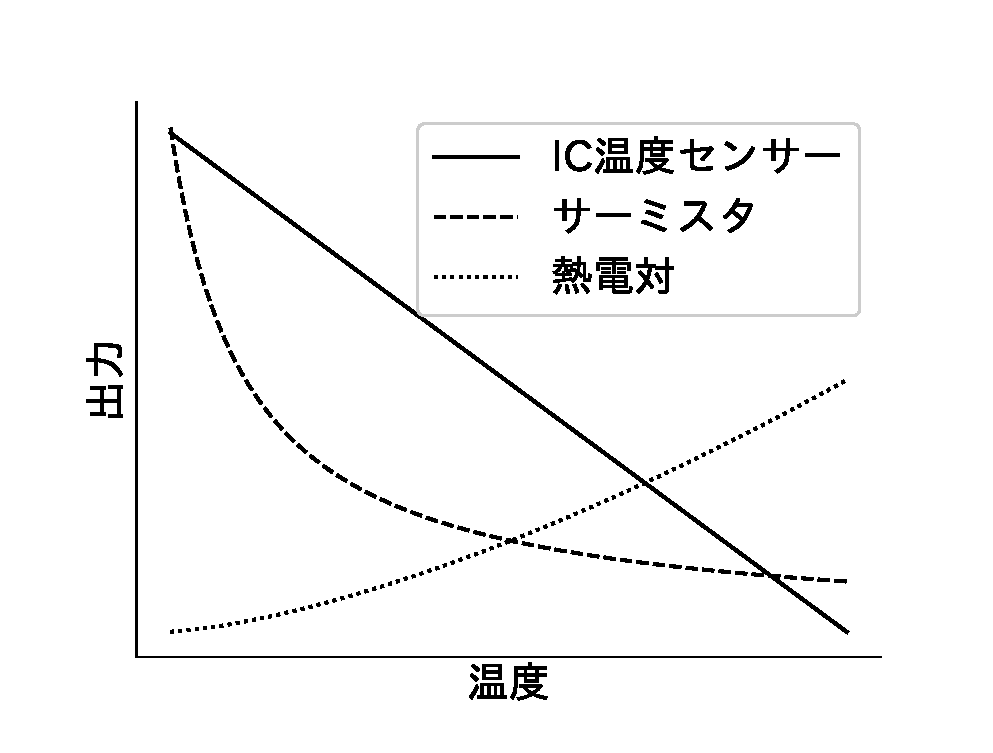
\includegraphics[width=1\hsize]{img/sensors.eps}
        \caption{各センサーの温度特性}
        \label{fig:sensors}
    \end{figure}

    図\ref{fig:sensors}でそれぞれ各センサーの特性の概形を比較している。
    IC温度センサーは他のセンサーより線形的な特性を持つことが見て取れる。
    この特長により、出力を処理せずにそのまま使用可能である。

\section{用途}
    IC温度センサーは、主に回路基盤の温度を制御する上でその監視に使われる。
    これは、電源さえあれば追加の回路なしで出力を得られるからである。
    さらに、IC温度センサーは応答が遅い欠点を持つが、
    回路の温度変化は緩慢であるため、適任である。

    また、後に記すようにIC温度センサーは他のセンサーと比べて安価であるため、
    サーミスタなど他のセンサーから置き換えられて使用されることもある。

\section{長所$\cdot$短所}
    最後に、IC温度センサーの長所と短所を挙げる。

    \paragraph{長所}
        \begin{itemize}
            \item アナログ、デジタル両出力が可能
            \item 低価格
            \item 出力を得るのに追加の回路を必要としない
            \item 出力が線形
            \item 経年劣化が少ない
        \end{itemize}

    \paragraph{短所}
        \begin{itemize}
            \item 対応温度の範囲が狭い
            \item 熱容量が小さく、自身の温度が上昇しやすい
            \item 応答が遅い
            \item 電源が必要
        \end{itemize}

\begin{thebibliography}{99}
    \bibitem{omega} 「集積回路温度センサー(ICセンサー)入門」 オメガエンジニアリング \\
        \url{https://www.jp.omega.com/prodinfo/Integrated-Circuit-Sensors.html}
        2020/6
    \bibitem{marutsu} 「IC温度センサ」 マルツエレック株式会社 \\
        \url{https://www.marutsu.co.jp/contents/shop/marutsu/mame/49.html}
    \bibitem{ablic1} 「温度センサICのご紹介」 エイブリック株式会社 \\
        \url{https://www.ablic.com/jp/semicon/products/sensor/temperature-sensor-ic/intro/}
    \bibitem{macnica} 温度センサの種類と特性 シリーズ第1回「熱電対、RTD、サーミスタの特性」
        株式会社マクニカ \\
        \url{https://www.macnica.co.jp/business/semiconductor/articles/texas_instruments/130361/}
    \bibitem{macnica} 温度センサの種類と特性 シリーズ第2回「半導体温度センサとは」
        株式会社マクニカ \\
        \url{https://www.macnica.co.jp/business/semiconductor/articles/texas_instruments/130365/}
    \bibitem{ablic2} 「LDOとは? リニアレギュレータとは?」 エイブリック株式会社 \\
        \url{https://www.ablic.com/jp/semicon/products/power-management-ic/voltage-regulator-ldo/intro/}
    \bibitem{ei} 「【ダイオード】順方向電圧の温度特性について」 Electrical Information \\
        \url{https://detail-infomation.com/diode-forward-voltage-temperature-characteristics/}
\end{thebibliography}
\end{document}